\documentclass[aspectratio=169]{beamer} % 16:9 aspect ratio for modern screens

% Theme settings
\usetheme[progressbar=foot]{metropolis} % Minimalist theme
\metroset{progressbar=frametitle} % Progress bar soll nur folien mit titel berücksichtigen?
\setbeamercolor{background canvas}{bg=white} % White background color

\makeatletter
    \setlength{\metropolis@progressinheadfoot@linewidth}{1.5pt}
\makeatother


\usefonttheme{professionalfonts} % Font theme

% Packages
\usepackage[T1]{fontenc}   % Font encoding
\usepackage[ngerman]{babel} % German language
\usepackage[sfdefault]{FiraSans} % For FiraSans font
\usepackage[backend=biber, style=authoryear-comp
, sorting=nyt]{biblatex} % For bibliography
\usepackage{csquotes} % Recommended for biblatex with babel/polyglossia
\usepackage{textgreek} % Greek letters in text mode (aus references von Citavi)
\usepackage{tikz}          % For drawing graphics

\usepackage{graphicx}       % For including images
\usepackage{amsmath, amssymb} % For math symbols

\usepackage[labelformat=empty]{caption}


% Bibliography settings
\addbibresource{references.bib} % Path to the bibliography file

% custom Citation commands
\DeclareCiteCommand{\citeauthortitle}
  {\usebibmacro{prenote}}
  {\usebibmacro{citeindex}%
   \printnames{labelname}%
   \setunit{\space\textendash\space}
   \printfield{title}}
  {\multicitedelim}
  {\usebibmacro{postnote}}

  \DeclareCiteCommand{\citeauthortitleurl}
  {\usebibmacro{prenote}}
  {\usebibmacro{citeindex}%
   \printnames{labelname}%
   \setunit{\space\textendash\space}
   \printfield{title}%
   \setunit{\addsemicolon\space}
   \printfield{url}}
  {\multicitedelim}
  {\usebibmacro{postnote}}

\DeclareCiteCommand{\parenciteauthortitle}
  {\usebibmacro{prenote}}
  {\bibopenparen\usebibmacro{citeindex}%
   \printnames{labelname}%
   \setunit{\space\textendash\space}% <- Hier wird das Trennzeichen ":" hinzugefügt
   \printfield{title}\bibcloseparen}
  {\multicitedelim}
  {\usebibmacro{postnote}}

\makeatletter
\renewcommand\footnotesize{\tiny}
\makeatother

\newcommand{\figcite}[1]{\\[-3mm]{\tiny Quelle: \cite{#1}}}
\newcommand{\figciteweb}[1]{\\[-3mm]{\tiny aus: \citeauthortitle{#1}}}
\newcommand{\figciteweburl}[1]{\\[-3mm]{\tiny aus: \citeauthortitleurl{#1}}}
  
% Title page settings
\title{Hadronen im Quarkmodell}
\subtitle{Wissenschaftliches Präsentieren}
\author{Florian Adamczyk}
\date{\today}

\begin{document}

    % Black slide
    \begin{frame}<handout:0>[plain, noframenumbering]
        \begin{tikzpicture}[remember picture, overlay]
            \fill[black] (current page.south west) rectangle (current page.north east);
        \end{tikzpicture}
    \end{frame}

    % Appetizer Slide
    \begin{frame}<handout:0>[noframenumbering, plain]{Eine Reise in den Zoo der Teilchen}
        \centering
        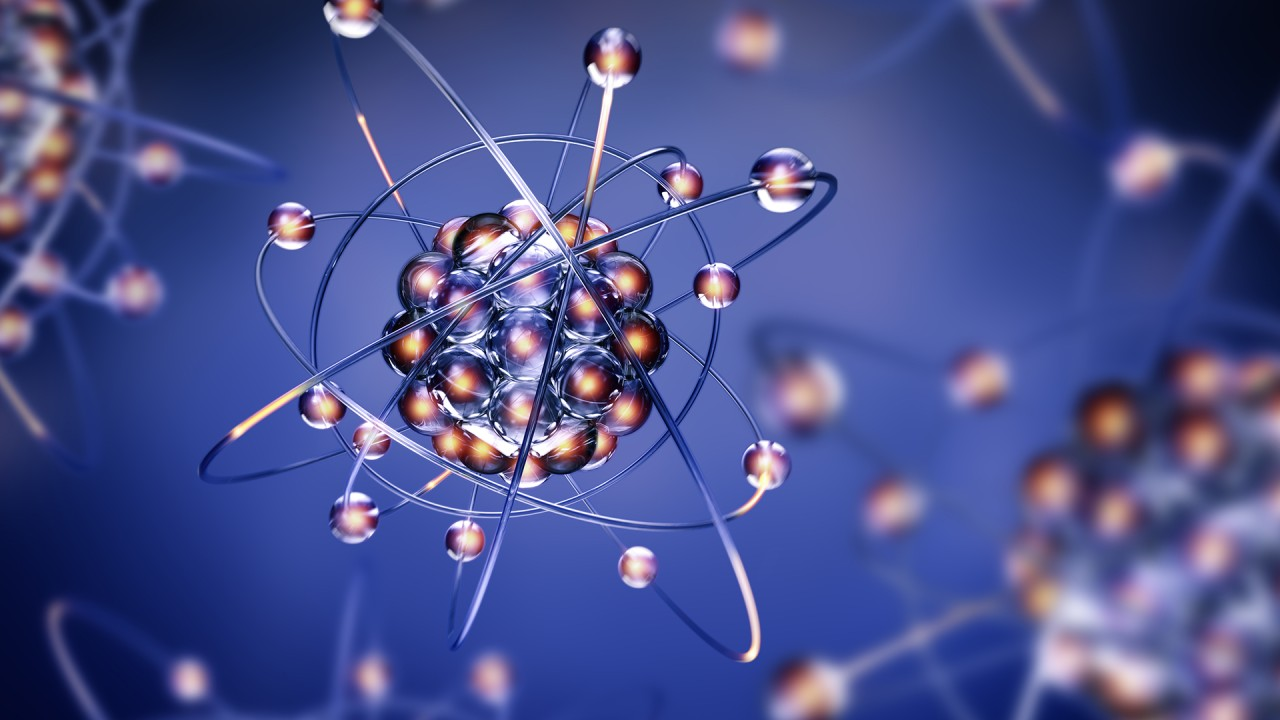
\includegraphics[width=\textwidth, height=0.9\textheight, keepaspectratio]{atom.jpg}
        \figciteweburl{Bonn.19.08.2021}
        % \vspace{0.5cm}
        % \begin{quote}
%{Stellen Sie sich vor, das Universum ist ein riesiger Zoo, bevölkert mit einer unglaublichen Vielfalt an exotischen Lebewesen – den Teilchen. Einige sind uns vertraut, wie Elektronen oder Protonen, aber es gibt auch faszinierende, kurzlebige Kreaturen. Eine Gruppe davon sind die Hadronen, die ich euch heute Vorstellen möchte.}
        % \end{quote}
    \end{frame}

    % Title Slide
    \begin{frame}[noframenumbering, plain]
        \vspace*{-0.6cm}
        \titlepage
        \vspace*{-1.6cm}
    \end{frame}
    
    % Table of Contents
    \begin{frame}{Gliederung}
      \setcounter{page}{1}      
        \tableofcontents
    \end{frame}
    
    \section{Das Standardmodell}
    \begin{frame}{Das Standardmodell der Elementarteilchen}
      \begin{figure}
        \centering
        \begin{minipage}{0.5\textwidth}
          \centering
          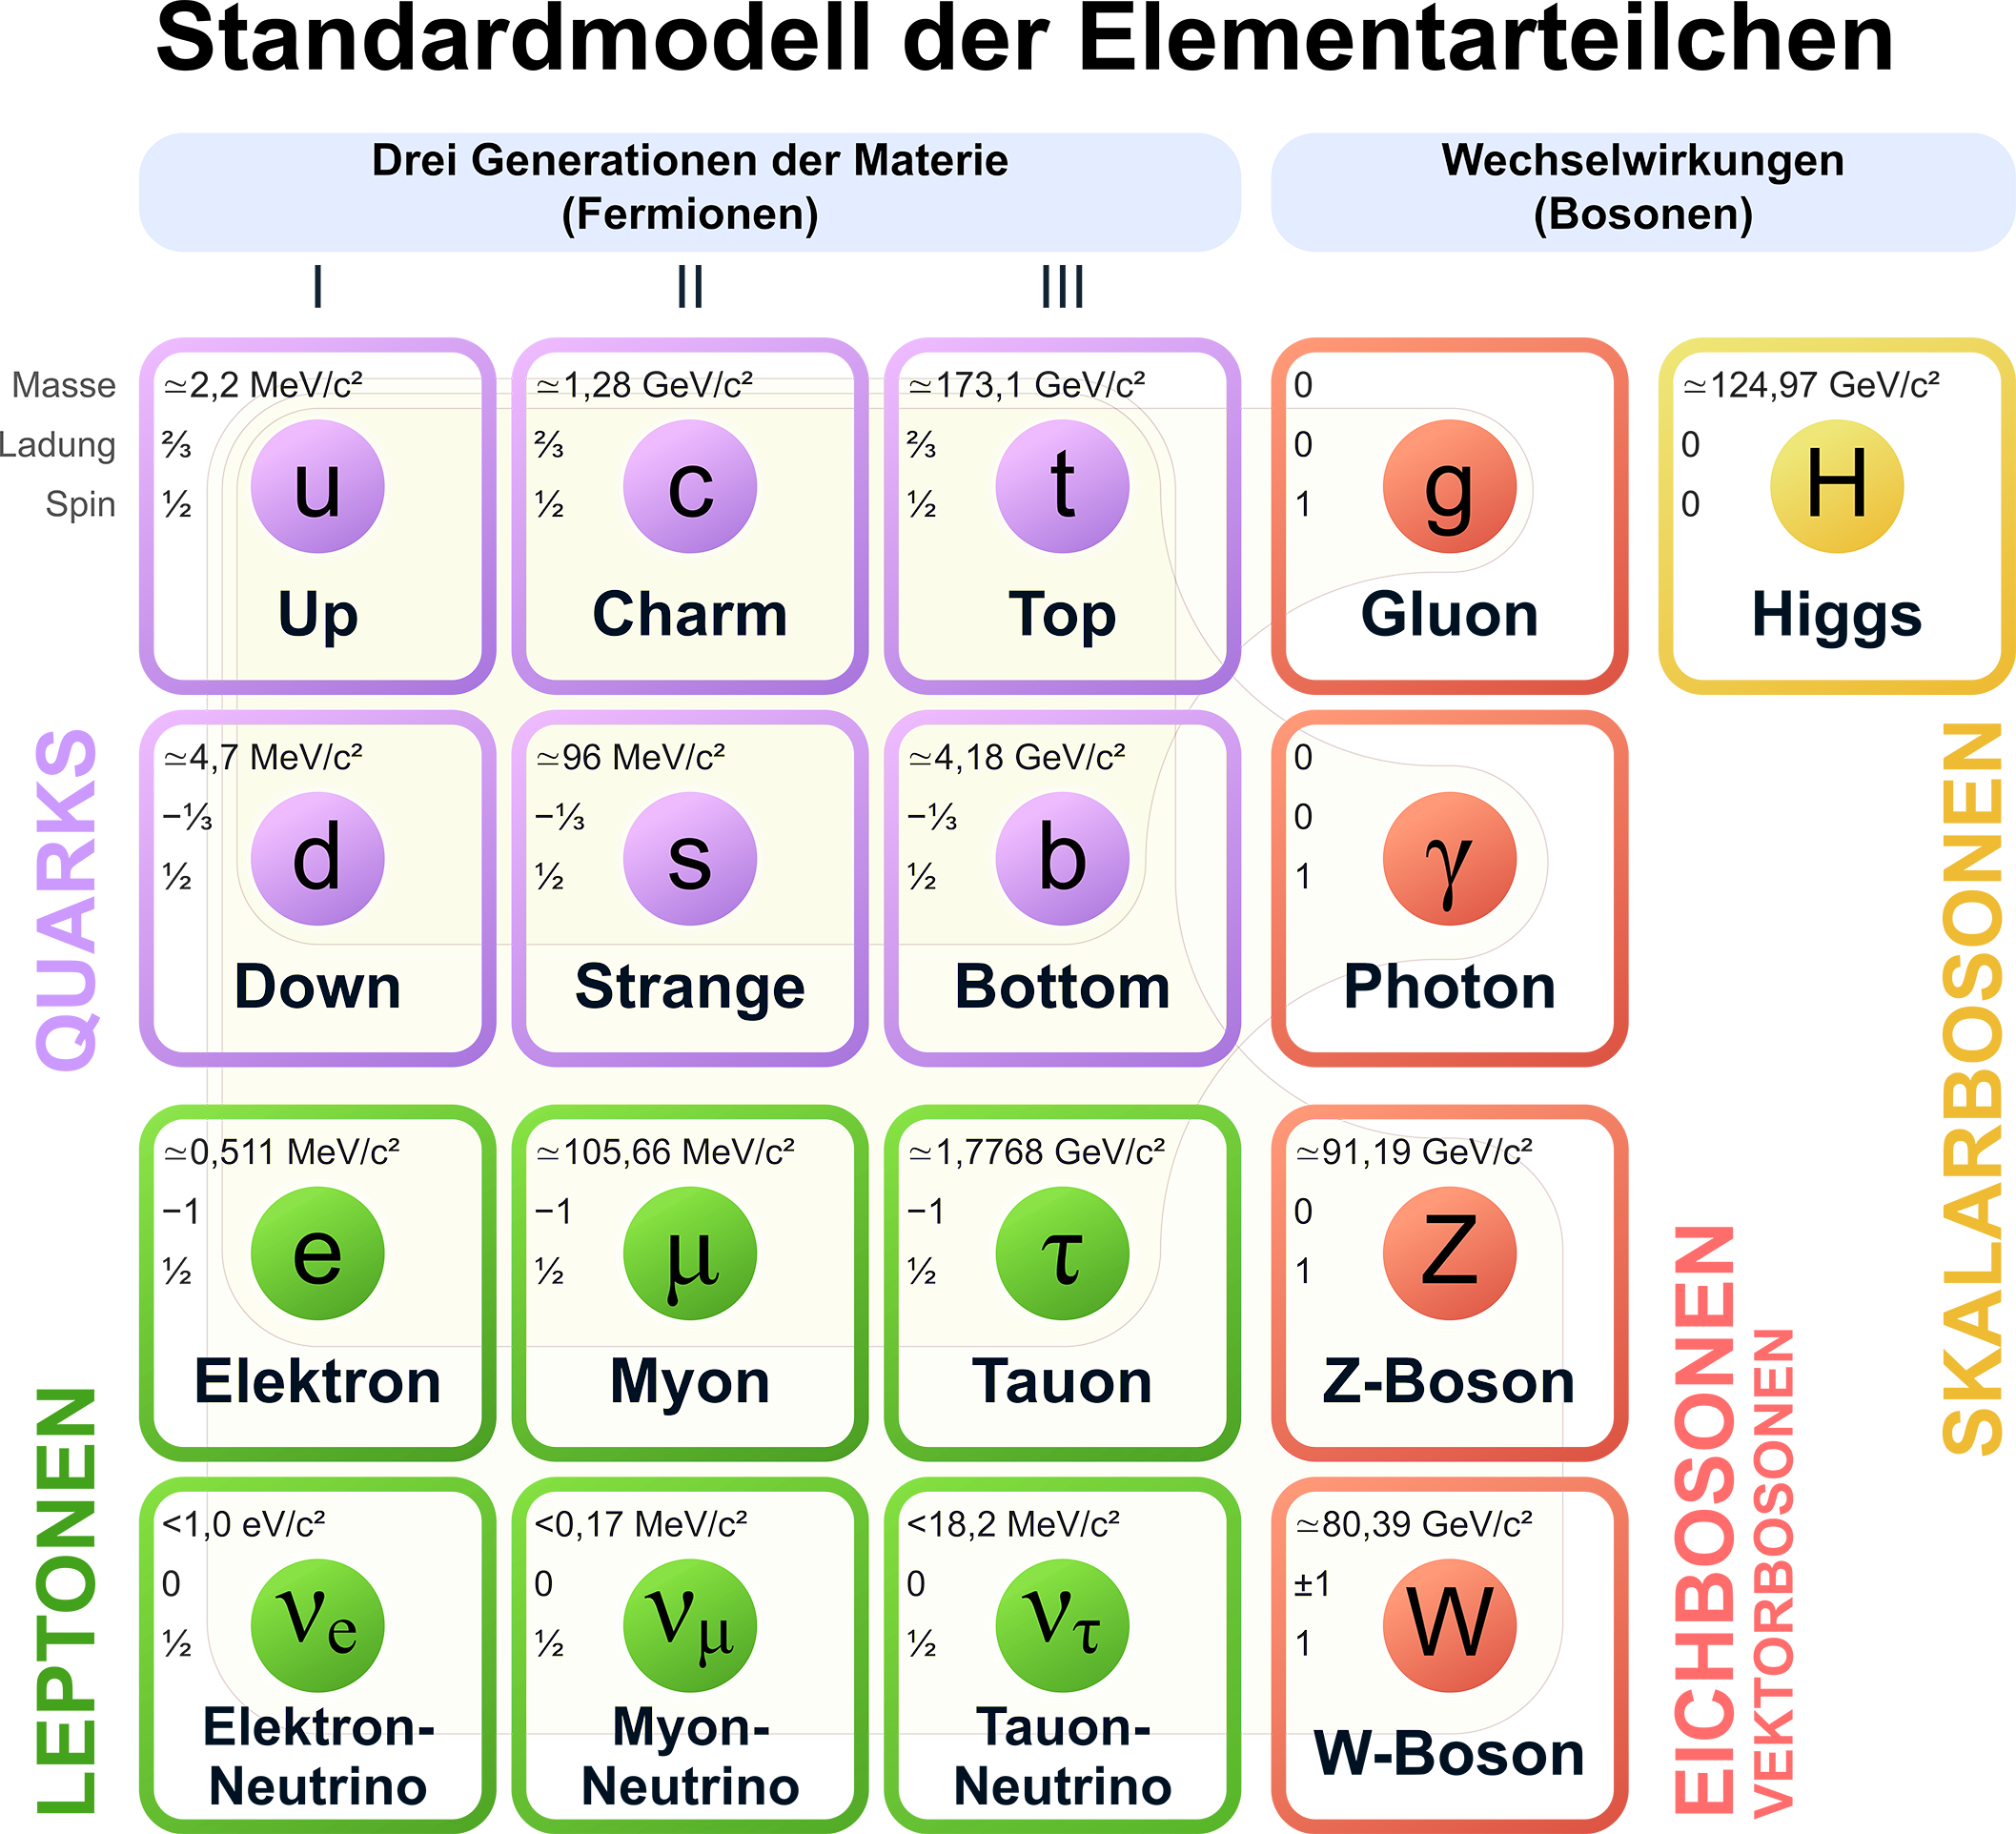
\includegraphics[width=\textwidth, keepaspectratio, height=0.85\textheight]{Standard_Model_of_Elementary_Particles_normal.png}\tiny
          \\\citeauthortitleurl{Wikipedia.Standardmodell}\end{minipage}
        \hfill \pause
        \begin{minipage}{0.48\textwidth}
          \begin{itemize}
            \item Beschreibt Elementarteilchen \& Wechselwirkungen \pause
            \item Fermionen (Quarks, Leptonen) \& Bosonen (Vektorbosonen, Higgs-Boson) \pause
            \item Starke, schwache \& elektromagnetische Wechselwirkung
          \end{itemize}
          \end{minipage}
      \end{figure}
    \end{frame}

    \subsection{Quarks}
    \begin{frame}{Quarks}
      \begin{figure}
        \centering
        \begin{minipage}{0.5\textwidth}
          \centering
          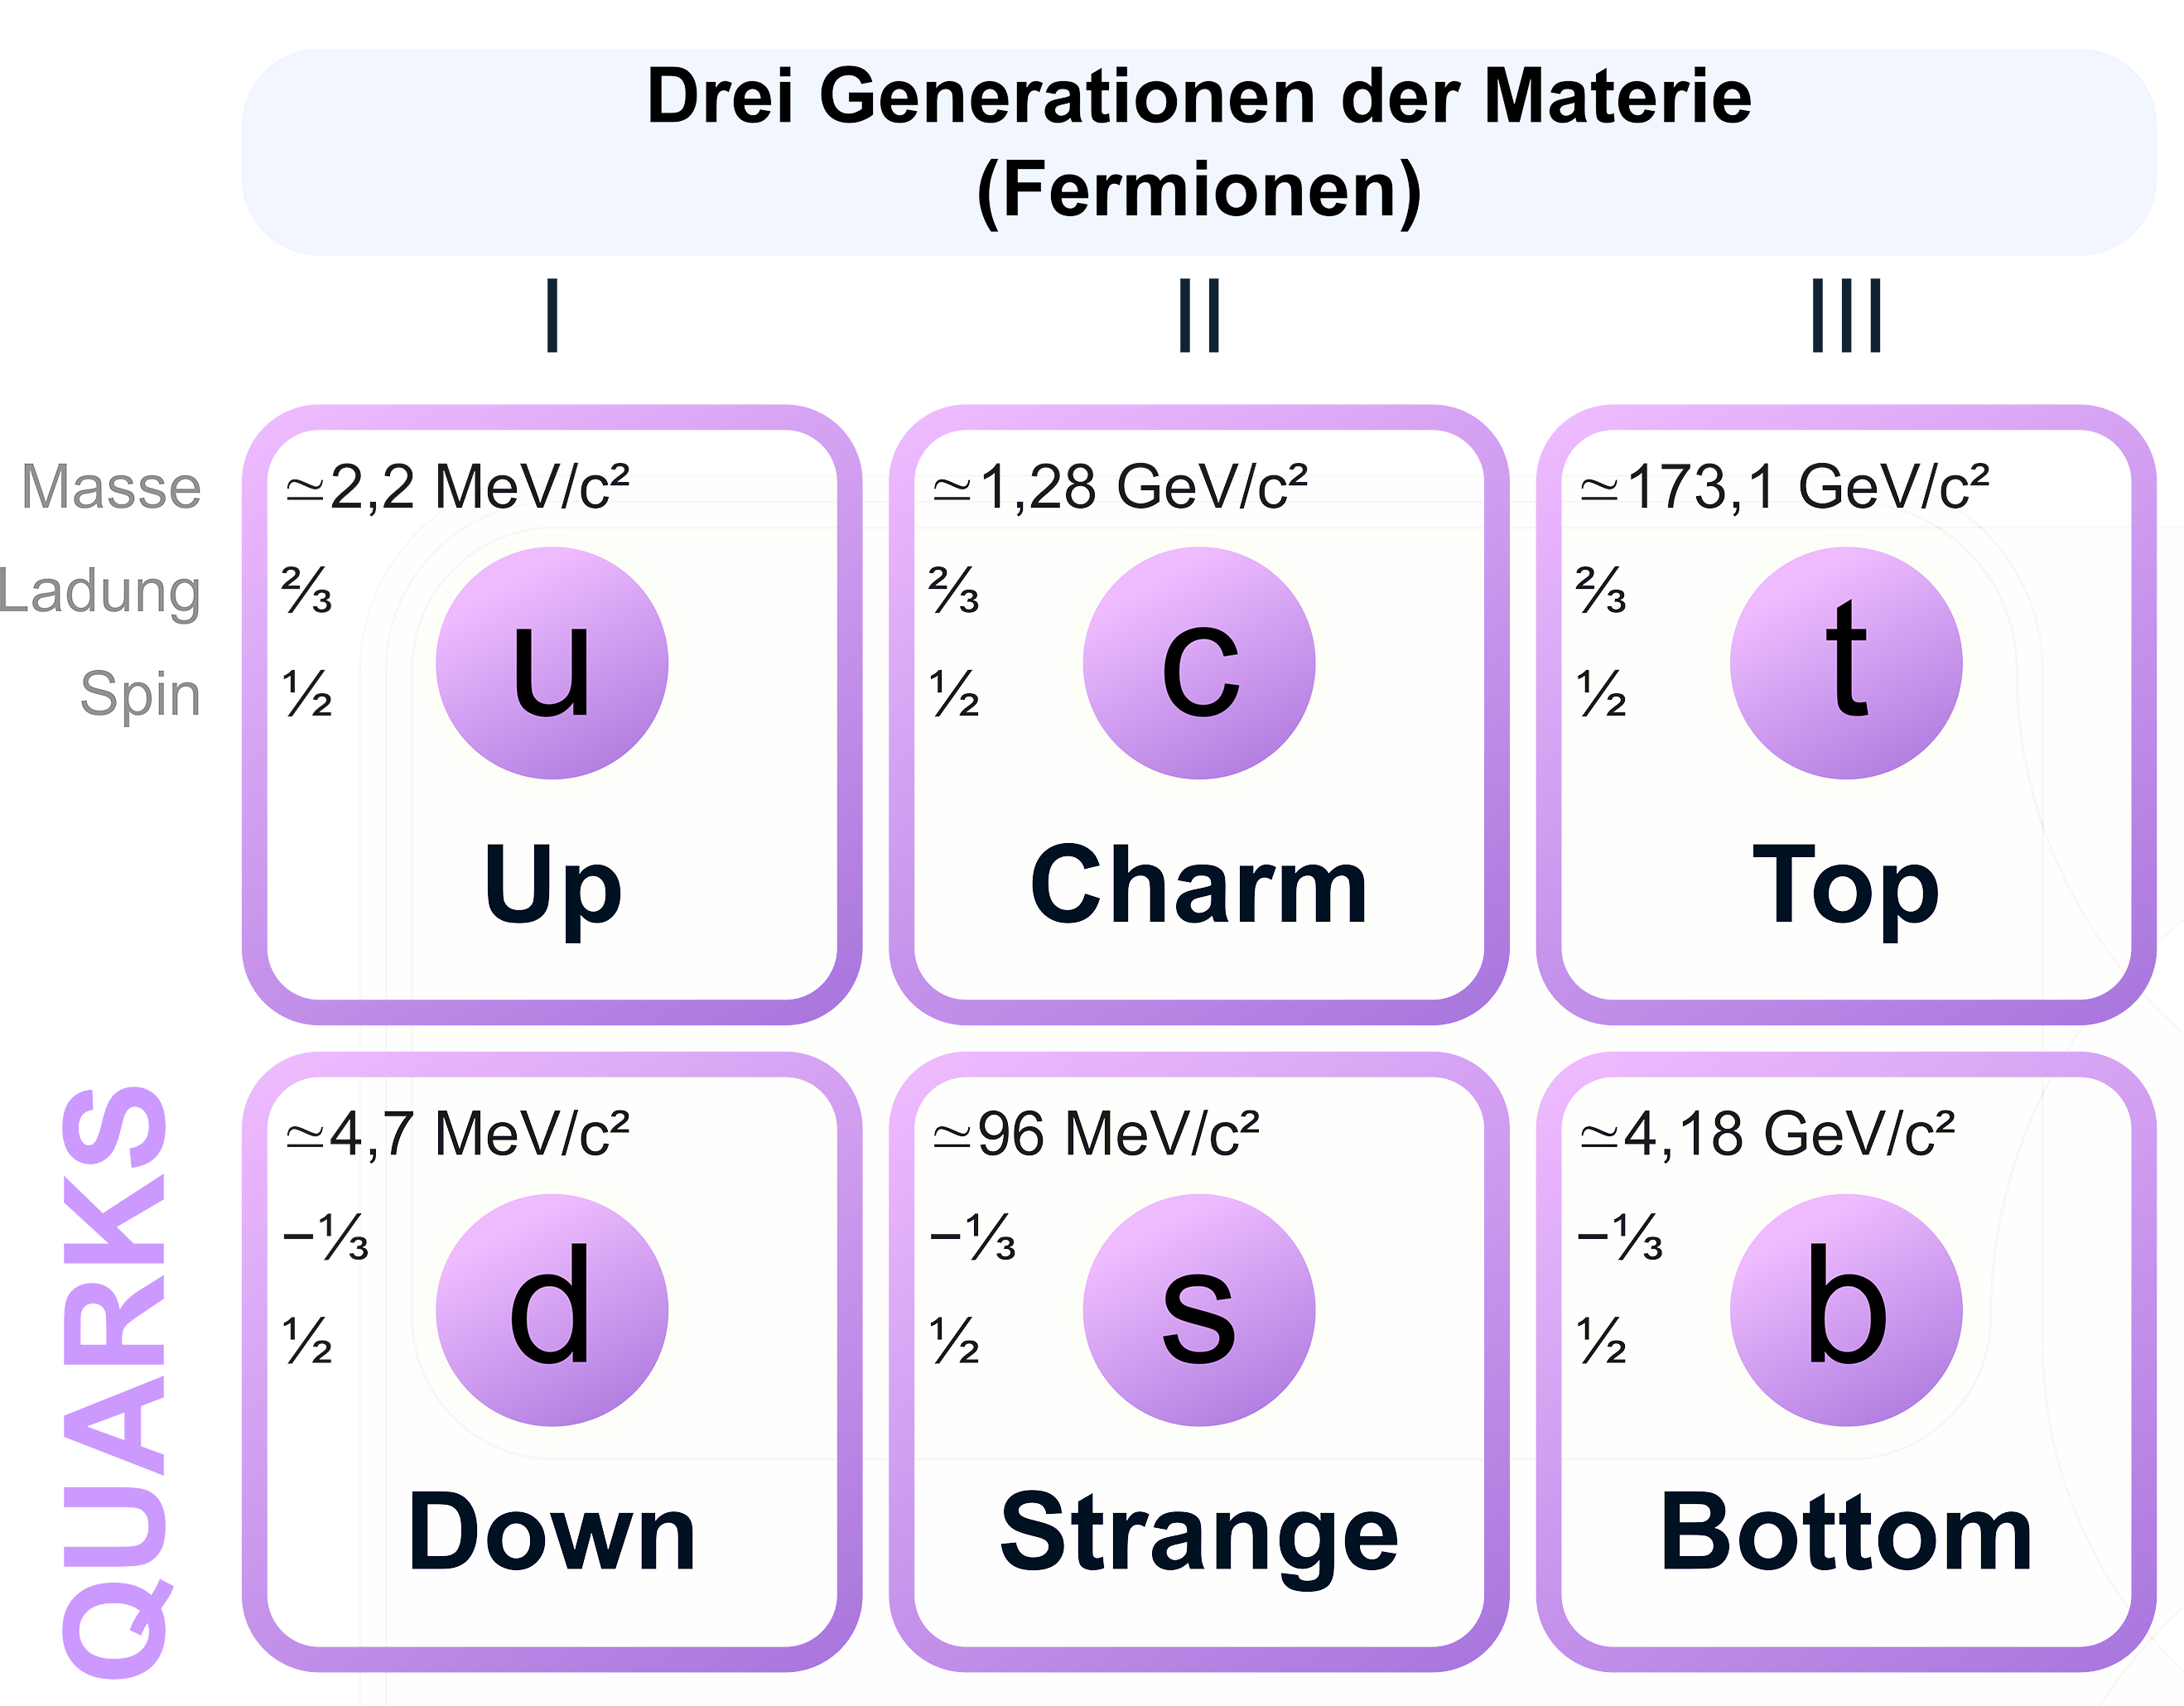
\includegraphics[width=\linewidth, keepaspectratio, height=\textheight]{Standard_Model_of_Elementary_Particles_zoom2.png}\tiny
          \\\citeauthortitleurl{Wikipedia.Standardmodell} \end{minipage}
        \hfill
        \begin{minipage}{0.48\textwidth}
          \begin{itemize}\pause
            \item Up, Charm, Top: $+\frac{2}{3}e$\pause
            \item Down, Strange, Bottom: $-\frac{1}{3}e$\pause
            \item Up, Down, Strange: leichtere Quarks\pause
            \item Charm, Bottom: schwerer\pause
            \item Top: schwerstes Quark \pause
            \item \textbf{Quarks nie isoliert!}
          \end{itemize}
          \end{minipage}
      \end{figure}
    \end{frame}

    \section{Hadronen}
    \subsection{Aufbau und Klassifizierung}
    \begin{frame}{Hadronen: Aufbau und Klassifizierung}
      \begin{itemize}
        \item <1-> Zusammengesetzt aus Quarks (durch starke WW gebunden)
        \item <3-> Baryonen (drei Quarks: Proton, Neutron, \dots)
        \item <4-> Mesonen ($q\bar{q}$, z.B. Pion, Kaon, \dots)
      \end{itemize}
      \centering
      \onslide<2->{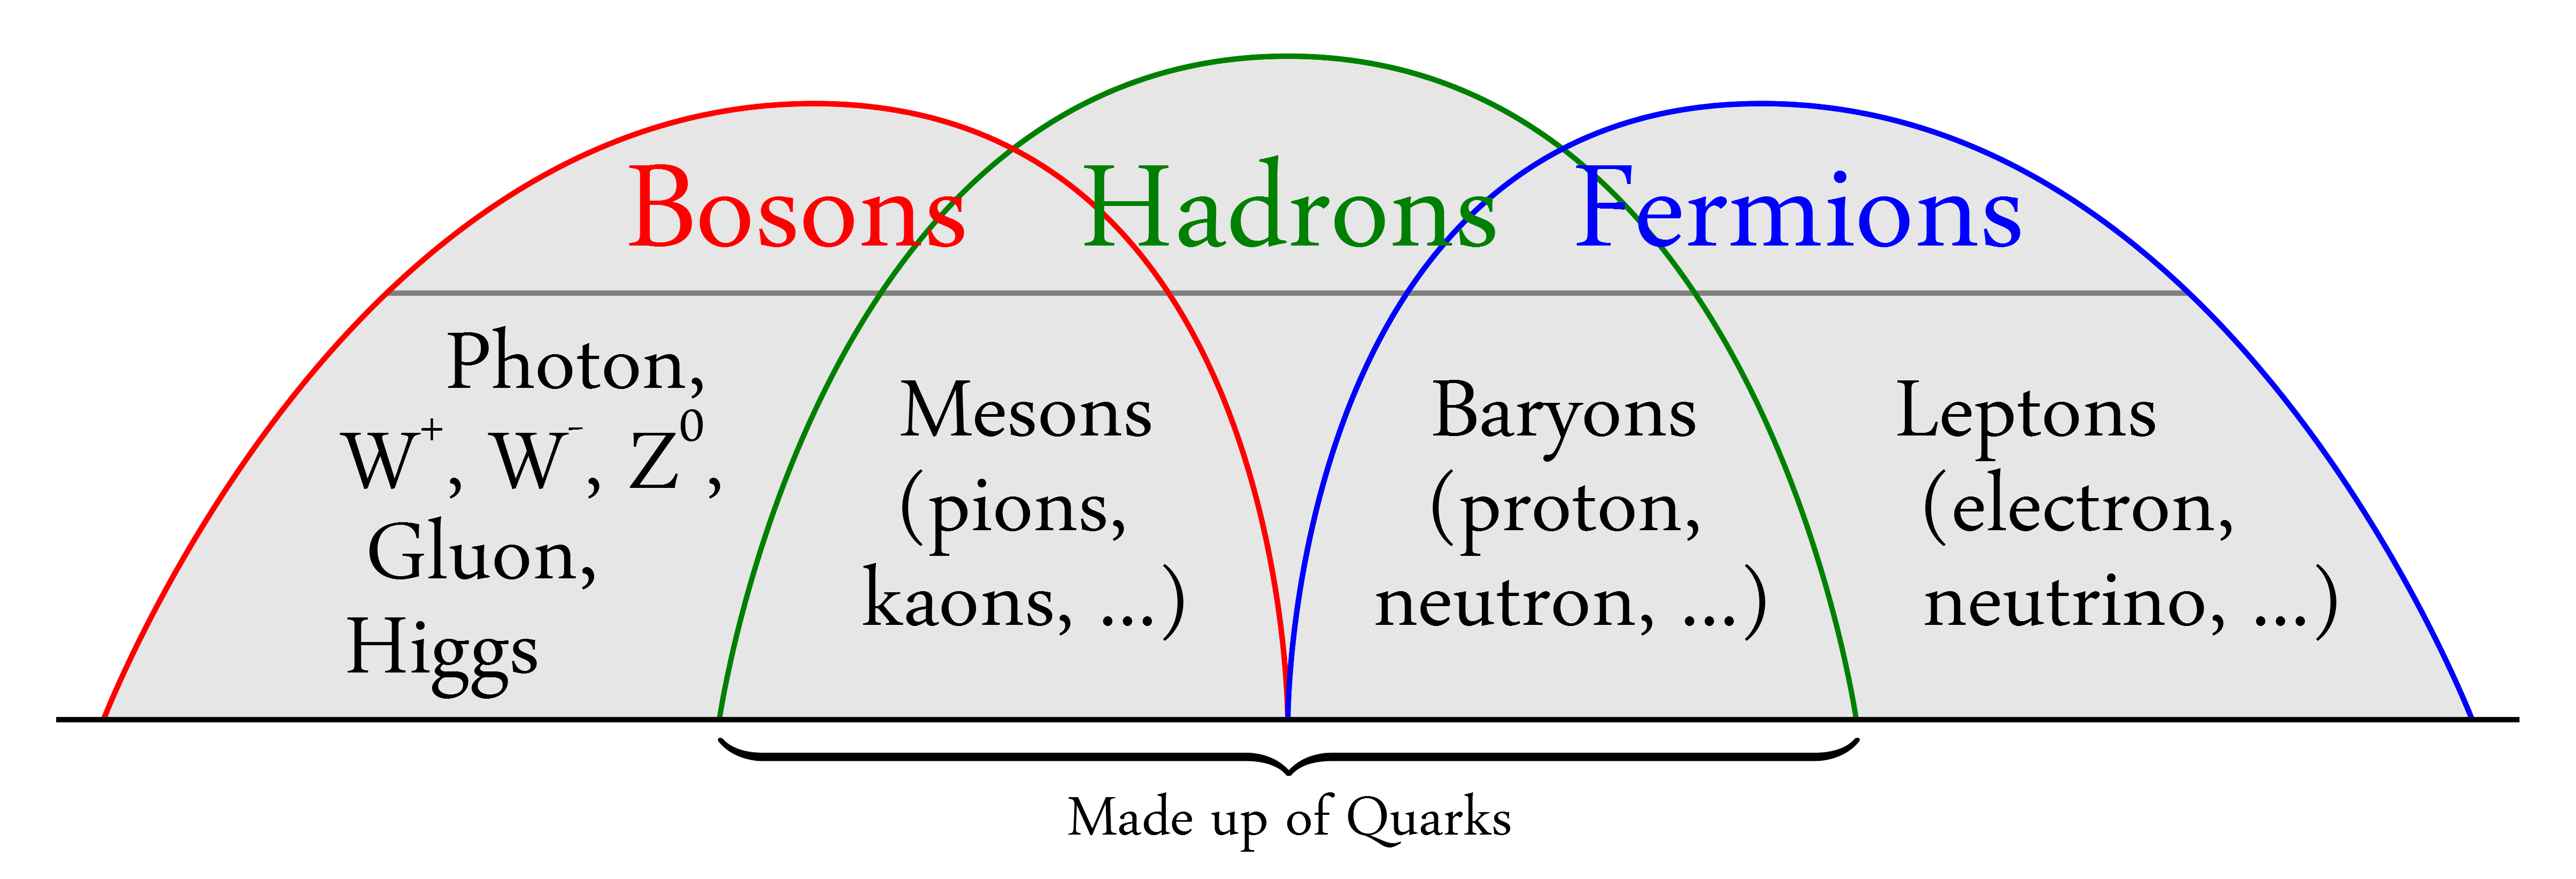
\includegraphics[width=\textwidth, height=0.4\textheight, keepaspectratio]{Bosons-Hadrons-Fermions-RGB-png2.png}}
      \onslide<2->{\figciteweburl{Wikipedia.Hadron}}
    \end{frame}

    \subsection{Das SU$_3$ Dekuplett}
    \begin{frame}{Das SU\(_3\) Dekuplett}
        \begin{minipage}{0.6\textwidth}
      \onslide<4->{\begin{figure}
            \centering
          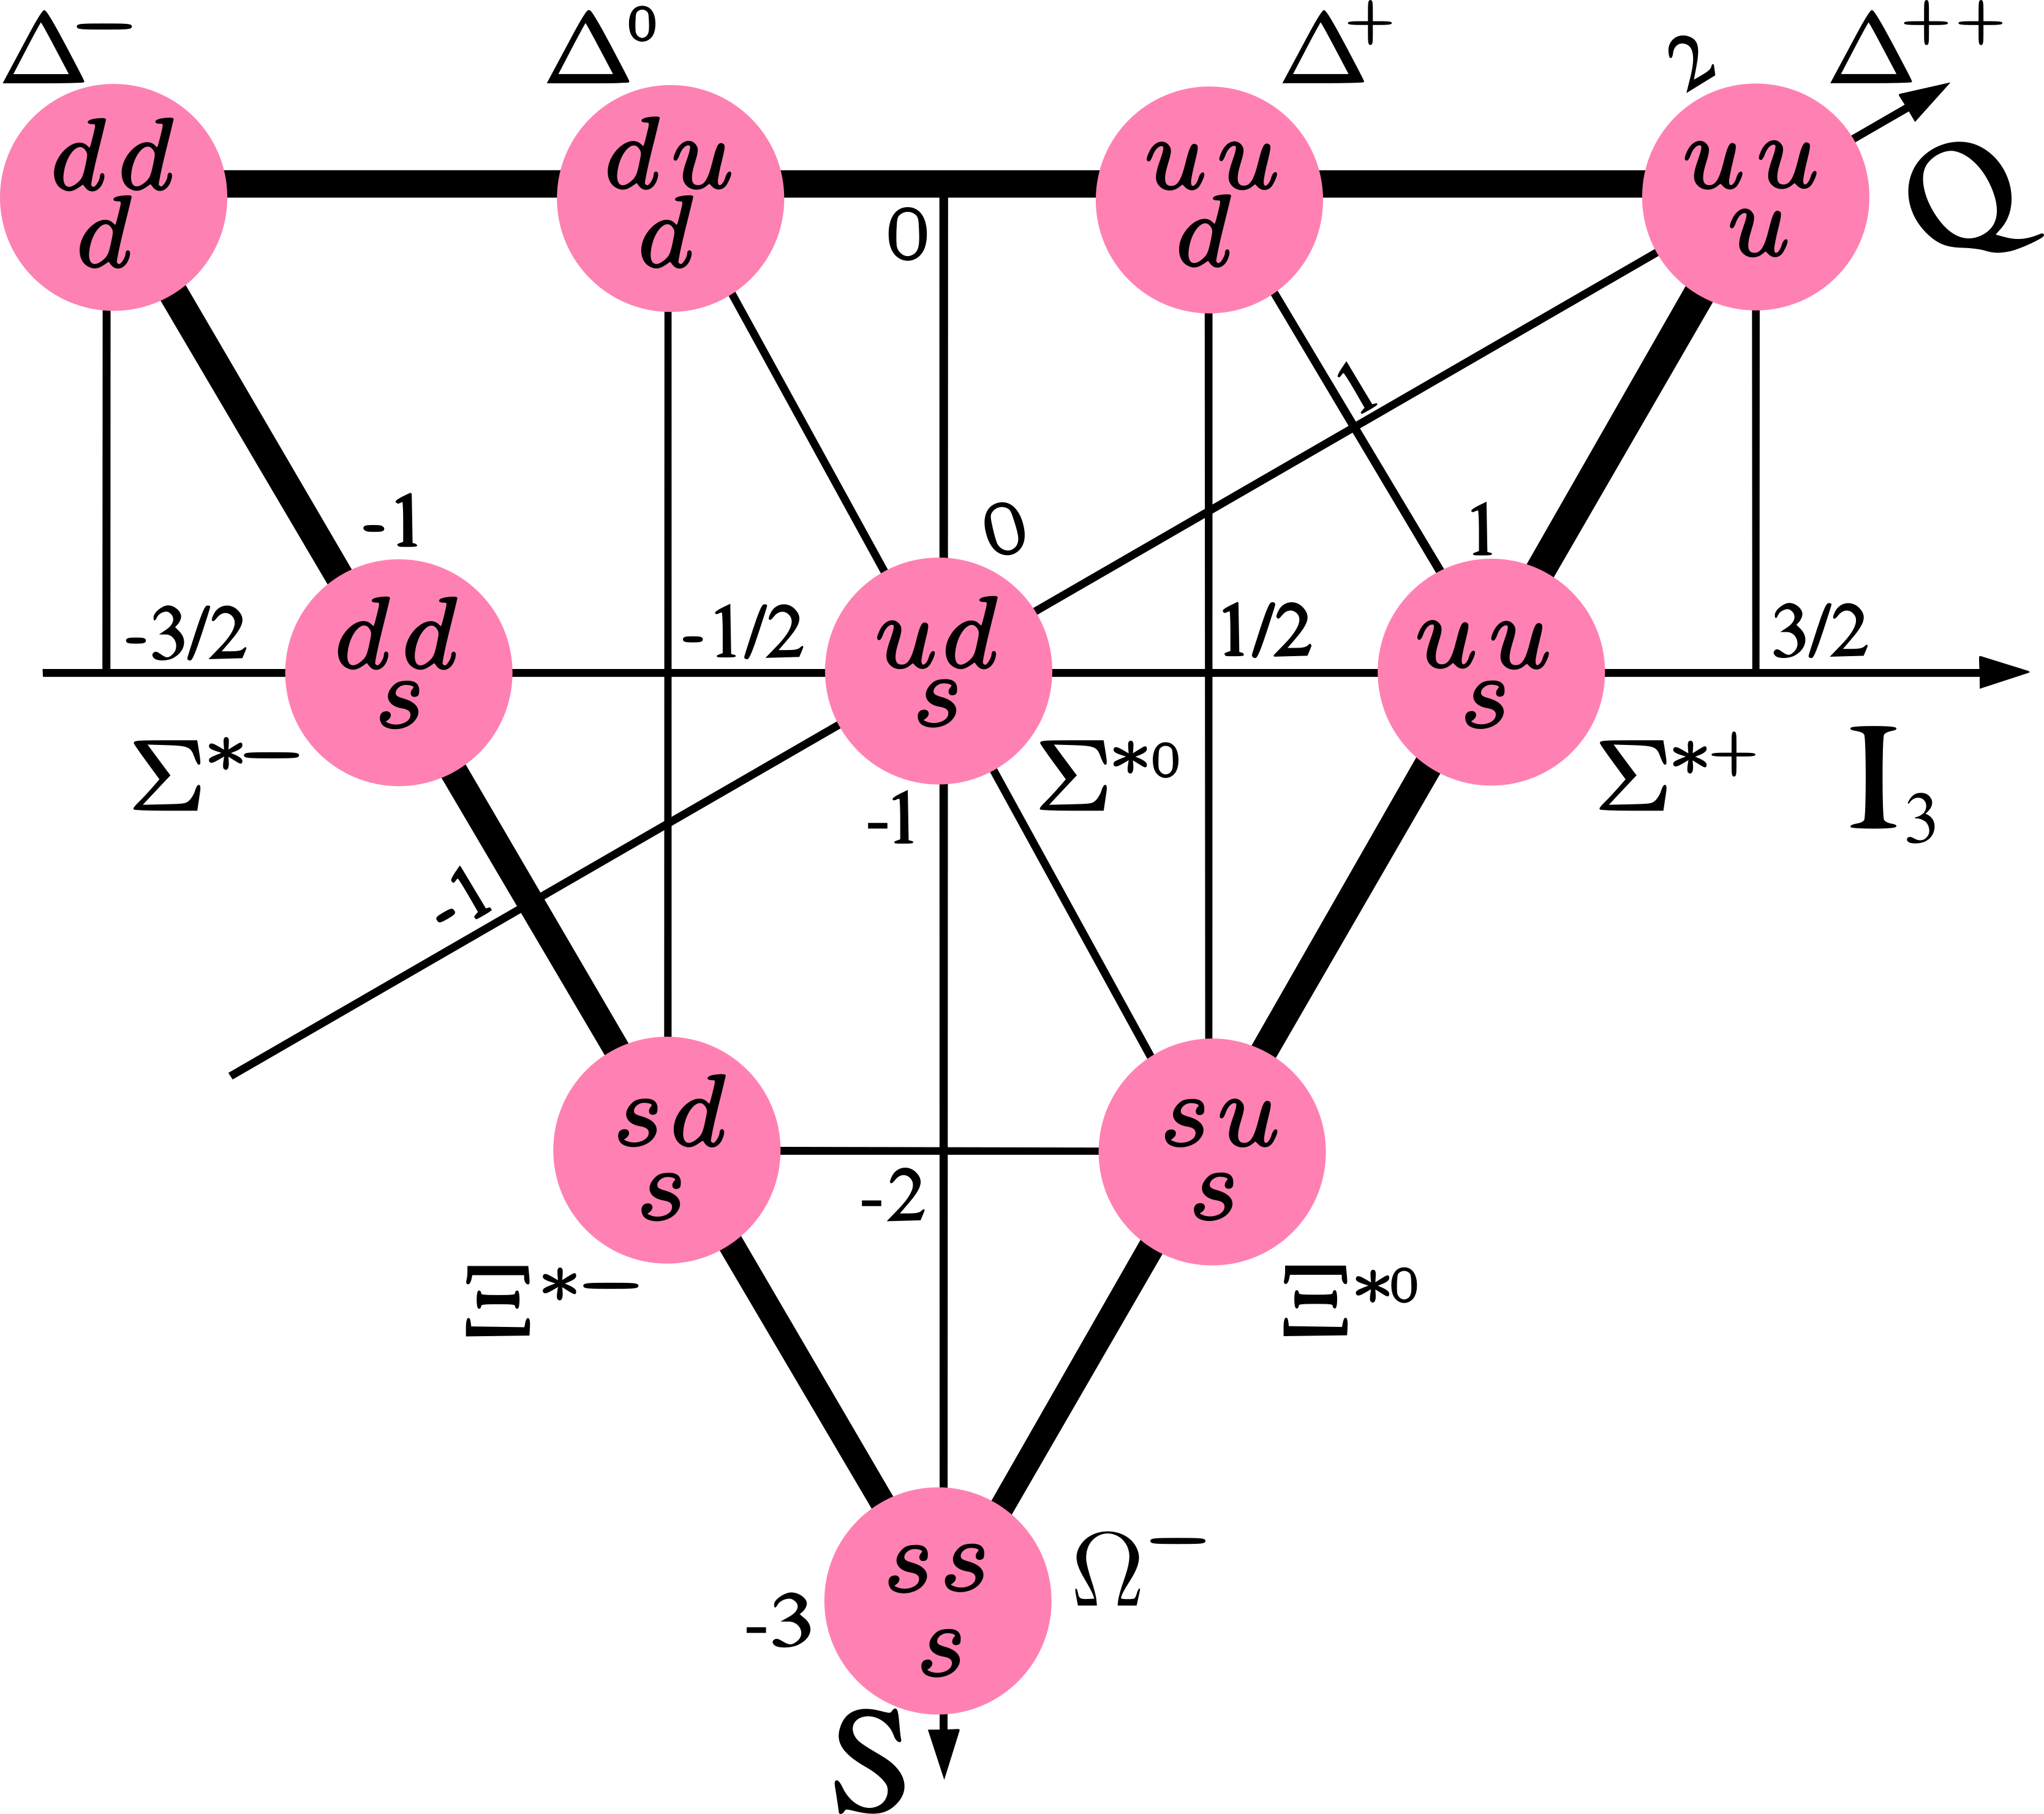
\includegraphics[width=\linewidth, keepaspectratio, height=0.8\textheight]{Baryon-decuplet-big.png}
          \tiny \\\citeauthortitle{Wikipedia.DeltaBaryon}, \citeurl{Wikipedia.DeltaBaryon}
      \end{figure}}
        \end{minipage}
        \hfill
        \begin{minipage}{0.38\textwidth}
                   
          \begin{itemize}
            \item<1-> S: Strangeness
            \item<2-> Q: Ladung
            \item<3-> I$_3$: Isospin % Grundzustand, parallele Spins und selben Falvour: Pauli Prinzip!!
          \end{itemize}
        \vspace{1em}
          
          \begin{tabular}{c|ccc}
            & up & down & strange\\
            \hline
            \onslide<1->{S & $0$ & $0$ & $-1$}\\
            \onslide<2->{Q & $+\frac{2}{3}$ & $-\frac{1}{3}$ & $-\frac{1}{3}$}\\
            \onslide<3->{I$_3$ & $\frac{1}{2}$ & $-\frac{1}{2}$ & $0$}
          \end{tabular}\\[1em]
                  
          \onslide<5->{$\rightarrow$\textbf{{ Einführung der \emph{Farbladung}}}}
        \end{minipage}
    \end{frame}
    
    \begin{frame}{Erweiterung des SU\(_3\) Dekupletts}
      \begin{minipage}{0.6\textwidth}
      \begin{figure}
        \centering
        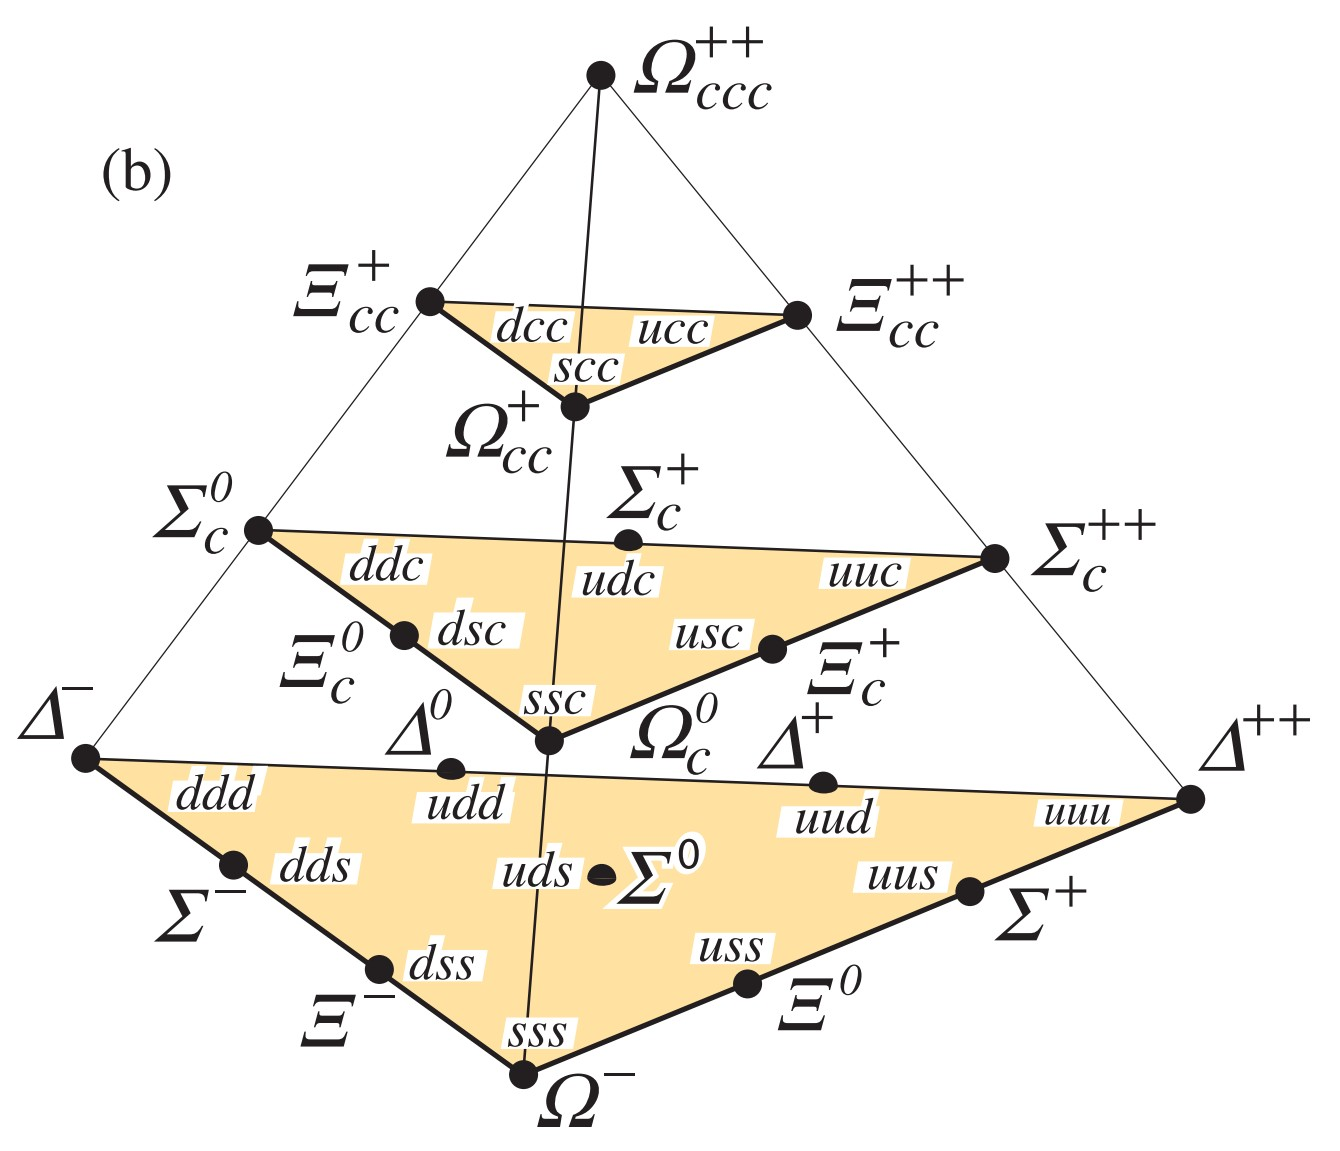
\includegraphics[width=\linewidth, height=0.7\textheight, keepaspectratio]{Images/594e59cc-d7ab-4a37-ad49-f782ae1831bc.jpg}
        \caption{Das 20-Plet mit einem SU$_3$ Dekuplett.\\\scriptsize\parencite{C.Amsler.2017}}
        \end{figure}
      \end{minipage}
      \hfill
      \begin{minipage}{0.38\textwidth}
        \begin{itemize}
          \item Erweiterung des SU$_3$ Dekupletts
          \item weitere Dimension: Charm
          \item Neue, schwere Hadronen
            \end{itemize}
          \end{minipage}
      \end{frame}

      \section{Geschichte: \emph{\glqq Erfindung\grqq} der Quarks}
              \begin{frame}{Gell-Mann: Zusammensetzung der Hadronen}
                \begin{figure}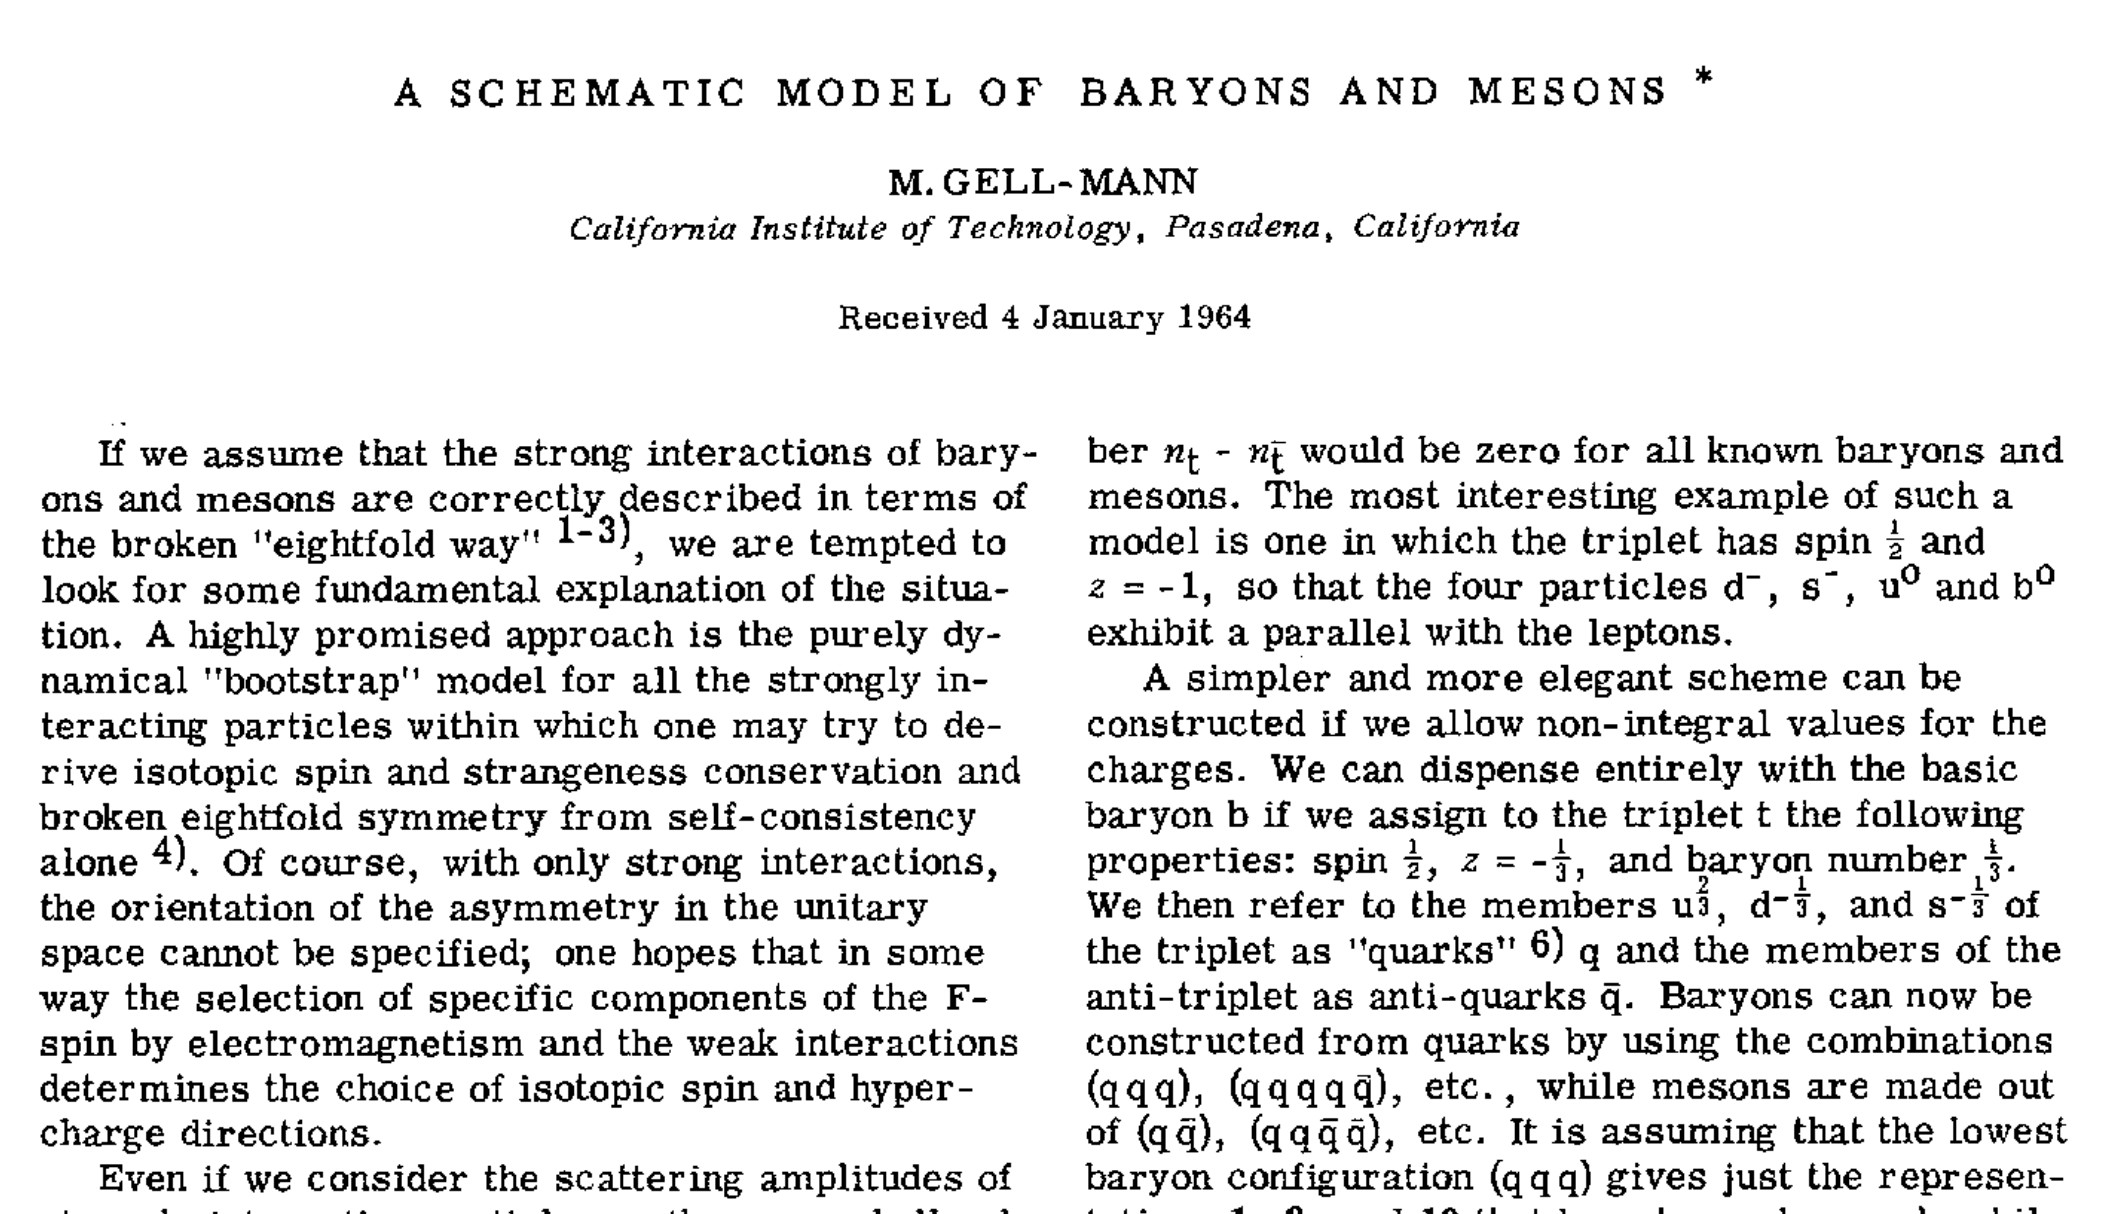
\includegraphics[height=0.85\textheight, width=\textwidth, keepaspectratio]{Images/8ad56d13-e301-4a37-be9c-7077ac16ce16.jpg}\\\small\cite[S.~214]{GellMann.1964,Zweig.1964}\end{figure}
                \begin{tikzpicture}[remember picture, overlay]\pause
            \fill[yellow, opacity=0.3] (7, 1.9) rectangle (12.8, 2.7);
                \end{tikzpicture}
    \end{frame}

    \section[Die Suche nach Pentaquarks]{Aktuelle Forschung}
    \subsection{Theoretische Vorhersagen}
    \begin{frame}{Pentaquarks: Theoretische Vorhersagen}
      \begin{minipage}{0.54\textwidth}
      \begin{itemize}
        \item Idee von \textcite{GellMann.1964} wurde durch \textcite{Hogaasen.1978, Strottman.1979} erweitert:
        \\
         \hspace{3mm} Theorie: $\mathrm{qqqq\bar{q}}$ \pause
         
         \item \textcite{Lipkin.1987} erfand den Begriff Pentaquark \pause
         \\[1em]
         \item Jedoch keine experimentellen Hinweise \pause % Das Problem war halt einfach die Energie!
      \end{itemize}
    \end{minipage}
\hfill
      \begin{minipage}{0.45\textwidth}
        \begin{figure}
          \centering
          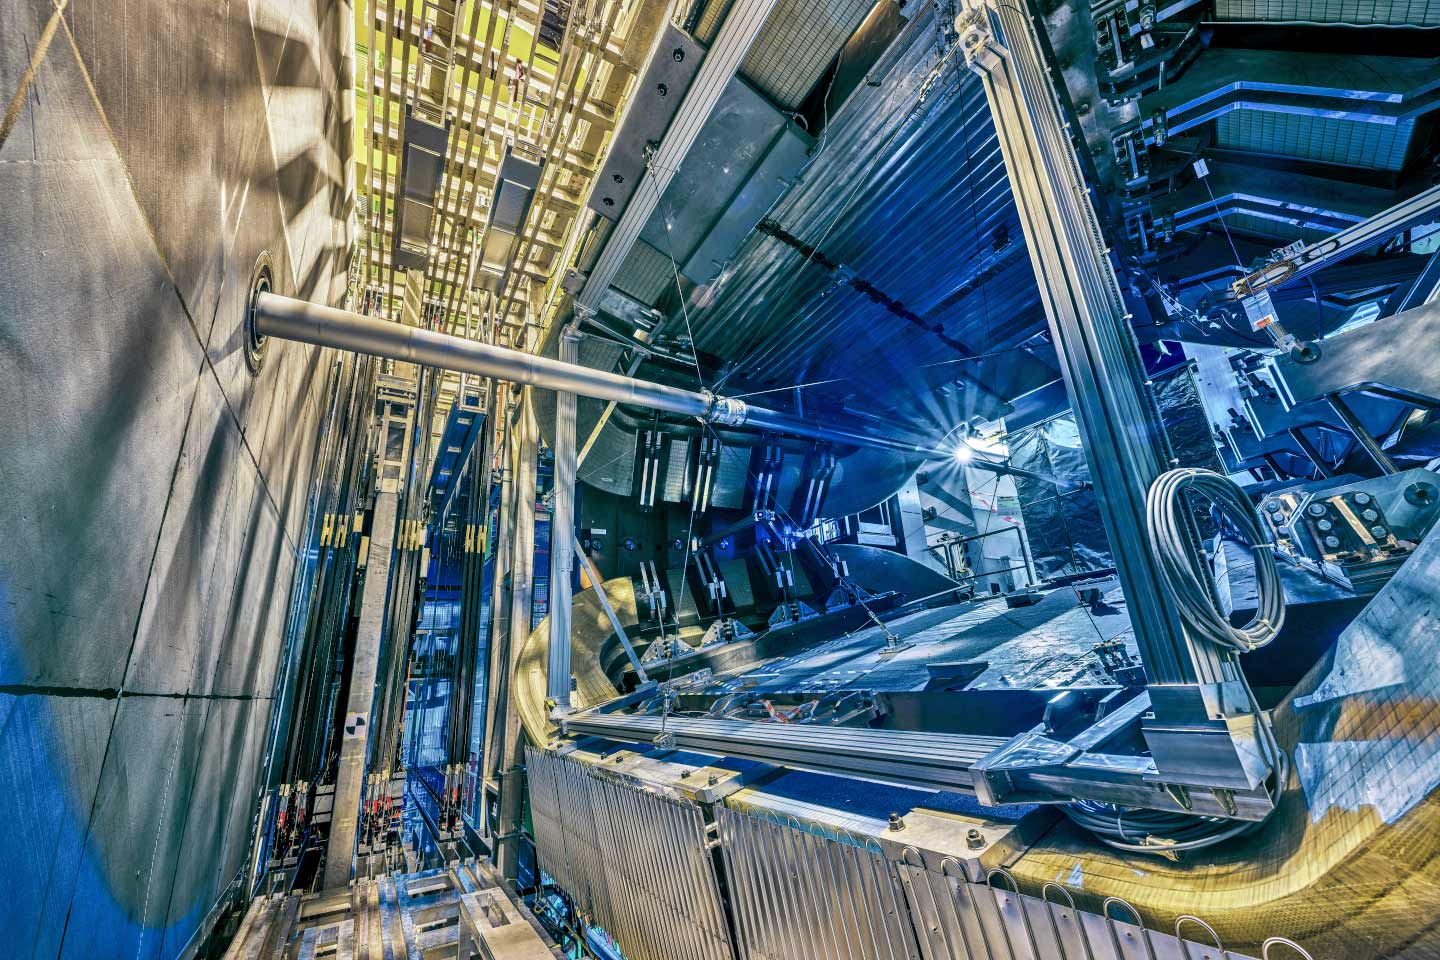
\includegraphics[width=\linewidth, height=\textheight, keepaspectratio]{fsp-LHCb-geoeffneter-detektor-blick-seite-2018-copyright-Brice-Ordan-CERN.jpg}
          \caption{Der LHCb Detektor am CERN\\\scriptsize\cite[Foto © Maximilien Brice, Julien Ordan | CERN ][]{.BMBF}}
        \end{figure}
      \end{minipage}
        \hfill
    \end{frame}

      \subsection{Experimentelle Entdeckung}
    \begin{frame}{LHCb: Untersuchung von $\mathrm{\Lambda_b^0}$ Zerfällen} %\emph{b steht für beauty}}
        \begin{minipage}{0.31\textwidth}
         \onslide<2->{ 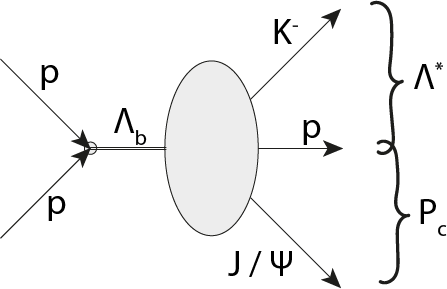
\includegraphics[width=\linewidth]{FeynmanDiag/Gesamt.png} 
          \onslide<-2>{\begin{tikzpicture}[remember picture, overlay]
            \fill[white] (3.5, 0.47) rectangle (4.4, 3.5); % white box, verdeckt beschriftung!
          \end{tikzpicture}}
          }
        \end{minipage}
        \hfill
        \begin{minipage}{0.67\textwidth}
          \begin{itemize}
            \item \textcite{Aaij.2015}: Untersuchung von $\mathrm{\Lambda_b^0} \to \mathrm{J}/\mathrm{\psi}\:\mathrm{K}^-\:\mathrm{p}$ Zerfällen.
            \item<3-> Zerfälle könnten minimalen Quarkanteil von $c\bar{c}uud$ enthalten. \\ $\rightarrow$ Charmonium Pentaquarks ($P_c$)
          \end{itemize}
        \end{minipage}
          \\
         \onslide<4->{\begin{figure}
          \centering
          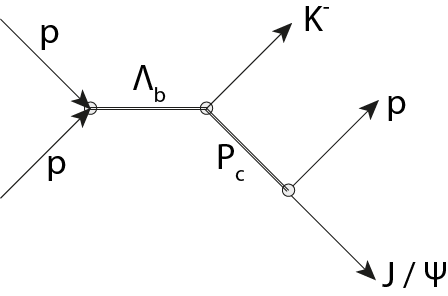
\includegraphics[width=0.3\textwidth]{FeynmanDiag/pentaquark.png}
          \hspace{2cm}
          \includegraphics[width=0.3\textwidth]{FeynmanDiag/lambda.png}
          \caption{Feynmandiagramme der Zerfallskanäle von $\mathrm{\Lambda_b^0} \to \mathrm{J}/\mathrm{\psi}\:\mathrm{K}^-\:\mathrm{p}$\\\tiny \emph{Eigene Darstellung nach Daten von \textcite{Aaij.2015}}}
      \end{figure}}
  \end{frame}


    \begin{frame}{Ergebnis der LHCb 2015 Messungen}
      \begin{minipage}{0.38\textwidth}
      \begin{figure}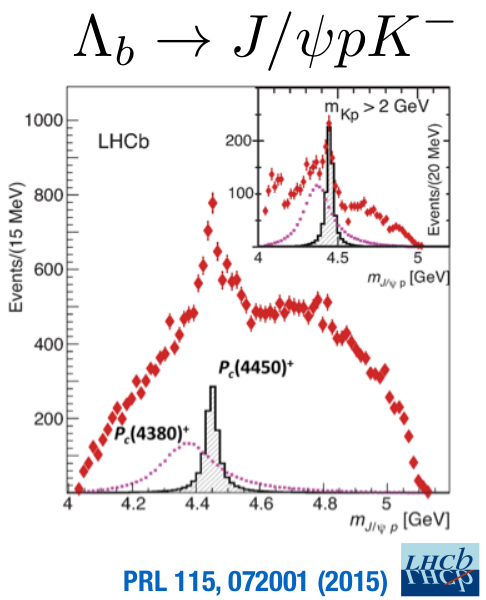
\includegraphics[width=\textwidth, height=0.8\textheight, keepaspectratio]{lhcb-pc4450.png}
        \\\cite{Aaij.2015}\end{figure}
      \end{minipage}
      \hfill
      \begin{minipage}{0.6\textwidth}
        \begin{itemize}
          \item Messung von $P_c^+(4380)$ und $P_c^+(4450)$
        \end{itemize}
        \vspace{2em}
        \begin{quote}\glqq The significance of each of these resonances is more than 9 standard deviations\grqq~\end{quote}~\cite[S.~1]{Aaij.2015}
      \end{minipage}
    \end{frame}

      \begin{frame}{LHCb 2019: Genauere Messung und weitere Pentaquarks}
        \begin{minipage}{0.4\textwidth}
          \begin{figure}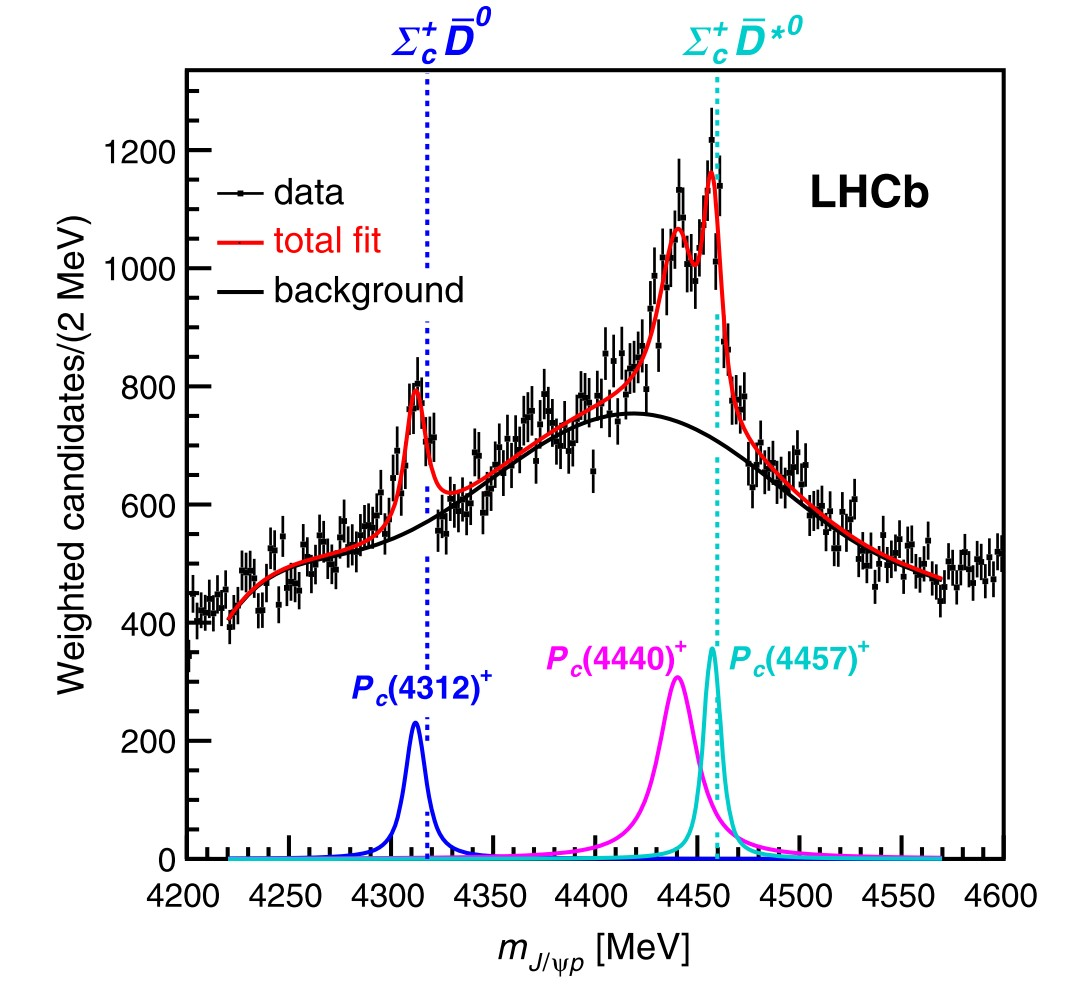
\includegraphics[width=\textwidth]{Images/76e29612-a8a4-4650-8573-5e331d33a362.jpg}
            \caption[S.~4]{\cite{Aaij.2019}}\end{figure}\pause
        \end{minipage}
        \hfill
        \begin{minipage}{0.58\textwidth}
          \begin{figure}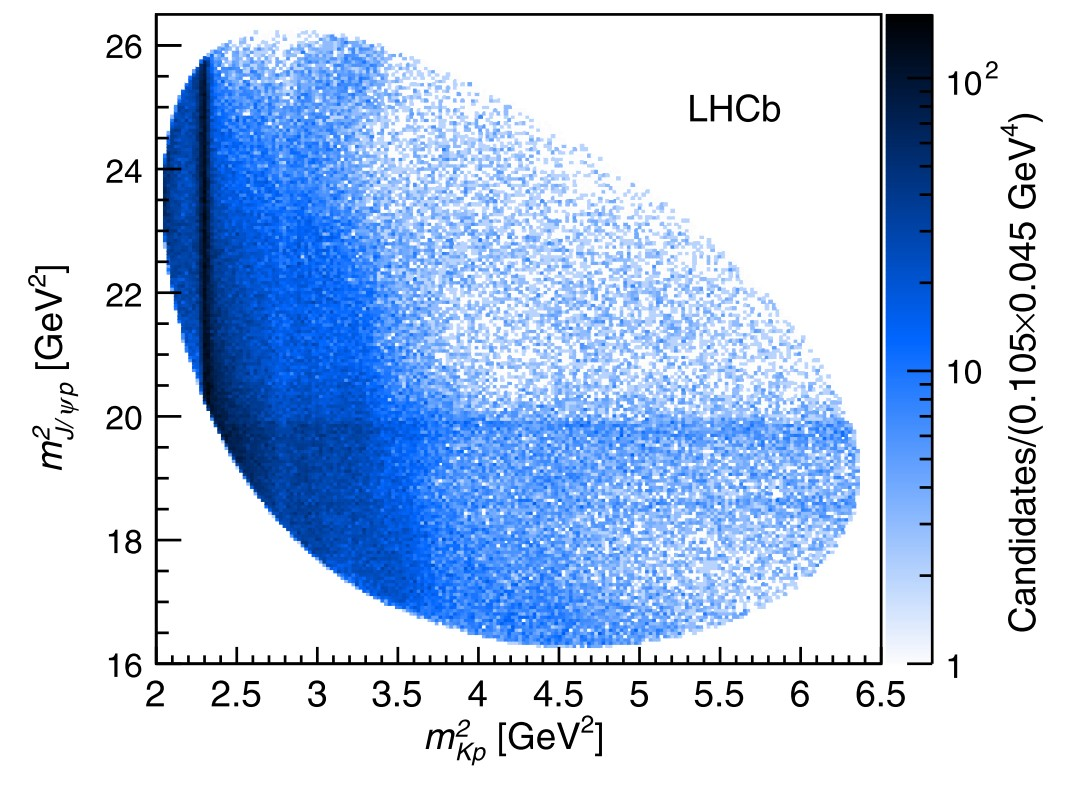
\includegraphics[width=\textwidth, height=0.5\textheight, keepaspectratio]{Images/e4479e29-be8d-4b9c-bfc4-f1747ace3818.jpg}\\[-3mm]{\scriptsize Dalitz-Plot der $\mathrm{\Lambda_b^0} \to \mathrm{J}/\mathrm{\psi}\:\mathrm{K}^-\:\mathrm{p}$ Kandidaten.}
          \end{figure}
          \centering
          \includegraphics[width=\textwidth, height=0.3\textheight, keepaspectratio]{FeynmanDiag/gesamt.png}
          \\[-2mm]
          {\scriptsize Eigene Darstellung des $\mathrm{\Lambda_b^0}$ Zerfalls.}
        \end{minipage}
      \end{frame}
    
    \begin{frame}{Fazit}
      \begin{itemize}
        \item Im \textbf{Standardmodell} werden Elementarteilchen und Wechselwirkungen beschrieben. \pause
        \item \textbf{Hadronen} bestehen aus 2, 4 (Mesonen), 3 oder 5 (Baryonen) Quarks.\pause
        \item Quarks sind unterschiedlich schwer und \textbf{nie isoliert}\pause
        \item \textbf{Pentaquarks} bestehen aus $\mathrm{qqqq\bar{q}}$ und wurden 2015 am LHCb entdeckt.
      \end{itemize}
      \centering
      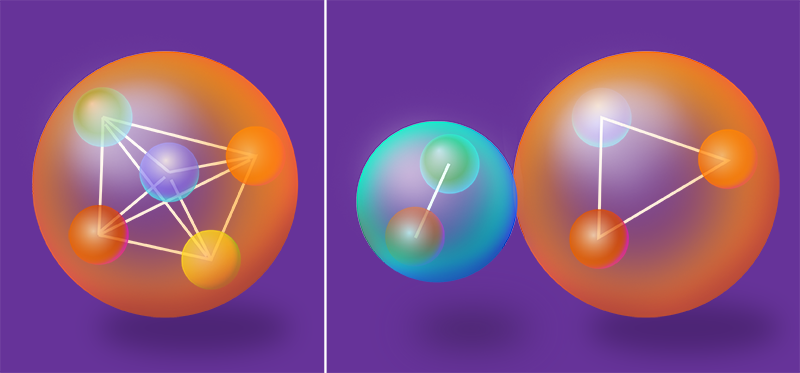
\includegraphics[width=\linewidth, height=0.46\textheight, keepaspectratio]{pentaquark model.png}
      \figciteweburl{KennethHicks.2015}
    \end{frame}

    % Thank You Slide
    \begin{frame}{Vielen Dank der Aufmerksamkeit!}
      \begin{center}
          \Huge Fragen?
      \end{center}
  \end{frame}

% Black slide
\begin{frame}<handout:0>[plain, noframenumbering]
  \begin{tikzpicture}[remember picture, overlay]
      \fill[black] (current page.south west) rectangle (current page.north east);
  \end{tikzpicture}
\end{frame}

  \begin{frame}<handout:0>[noframenumbering, plain, allowframebreaks]{Anhang}
      \begin{minipage}{0.4\textwidth}
        \textbf{Quarkzusammensetzung}
        \begin{itemize}
          \item $\mathrm{p = uud}$
          \item $\mathrm{K^- = s\bar{u}}$
          \item $\mathrm{\Lambda_b^0 = udb}$
          \item $\mathrm{\Lambda^* = uds}$
          \item $\mathrm{J/\psi = c\bar{c}}$
          \item $\mathrm{P_c^+ = c\bar{c}uud}$
        \end{itemize}
      \end{minipage}
      \hfill
      \begin{minipage}{0.58\textwidth}
        \begin{figure}
          \centering
          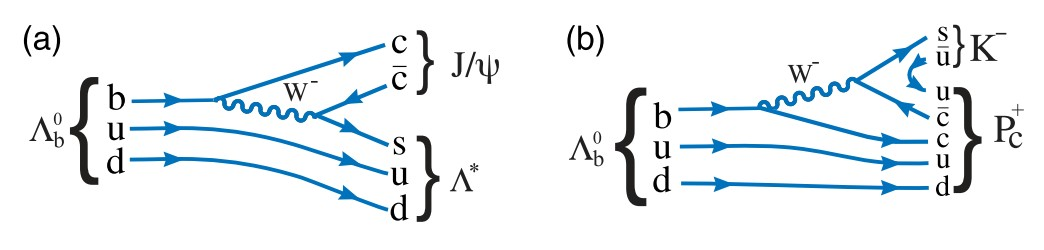
\includegraphics[width=\linewidth, height=0.5\textheight, keepaspectratio]{Images/98cb82e8-f82b-43ad-8d90-3c7881558f42.jpg}
          \caption{Feynman-Diagramm für $\mathrm{\Lambda_b^0} \to \mathrm{J}/\mathrm{\psi}\:\mathrm{K}^-\:\mathrm{p}$\\\scriptsize\cite{Aaij.2015}}
        \end{figure}
      \end{minipage}
      
    \pagebreak
      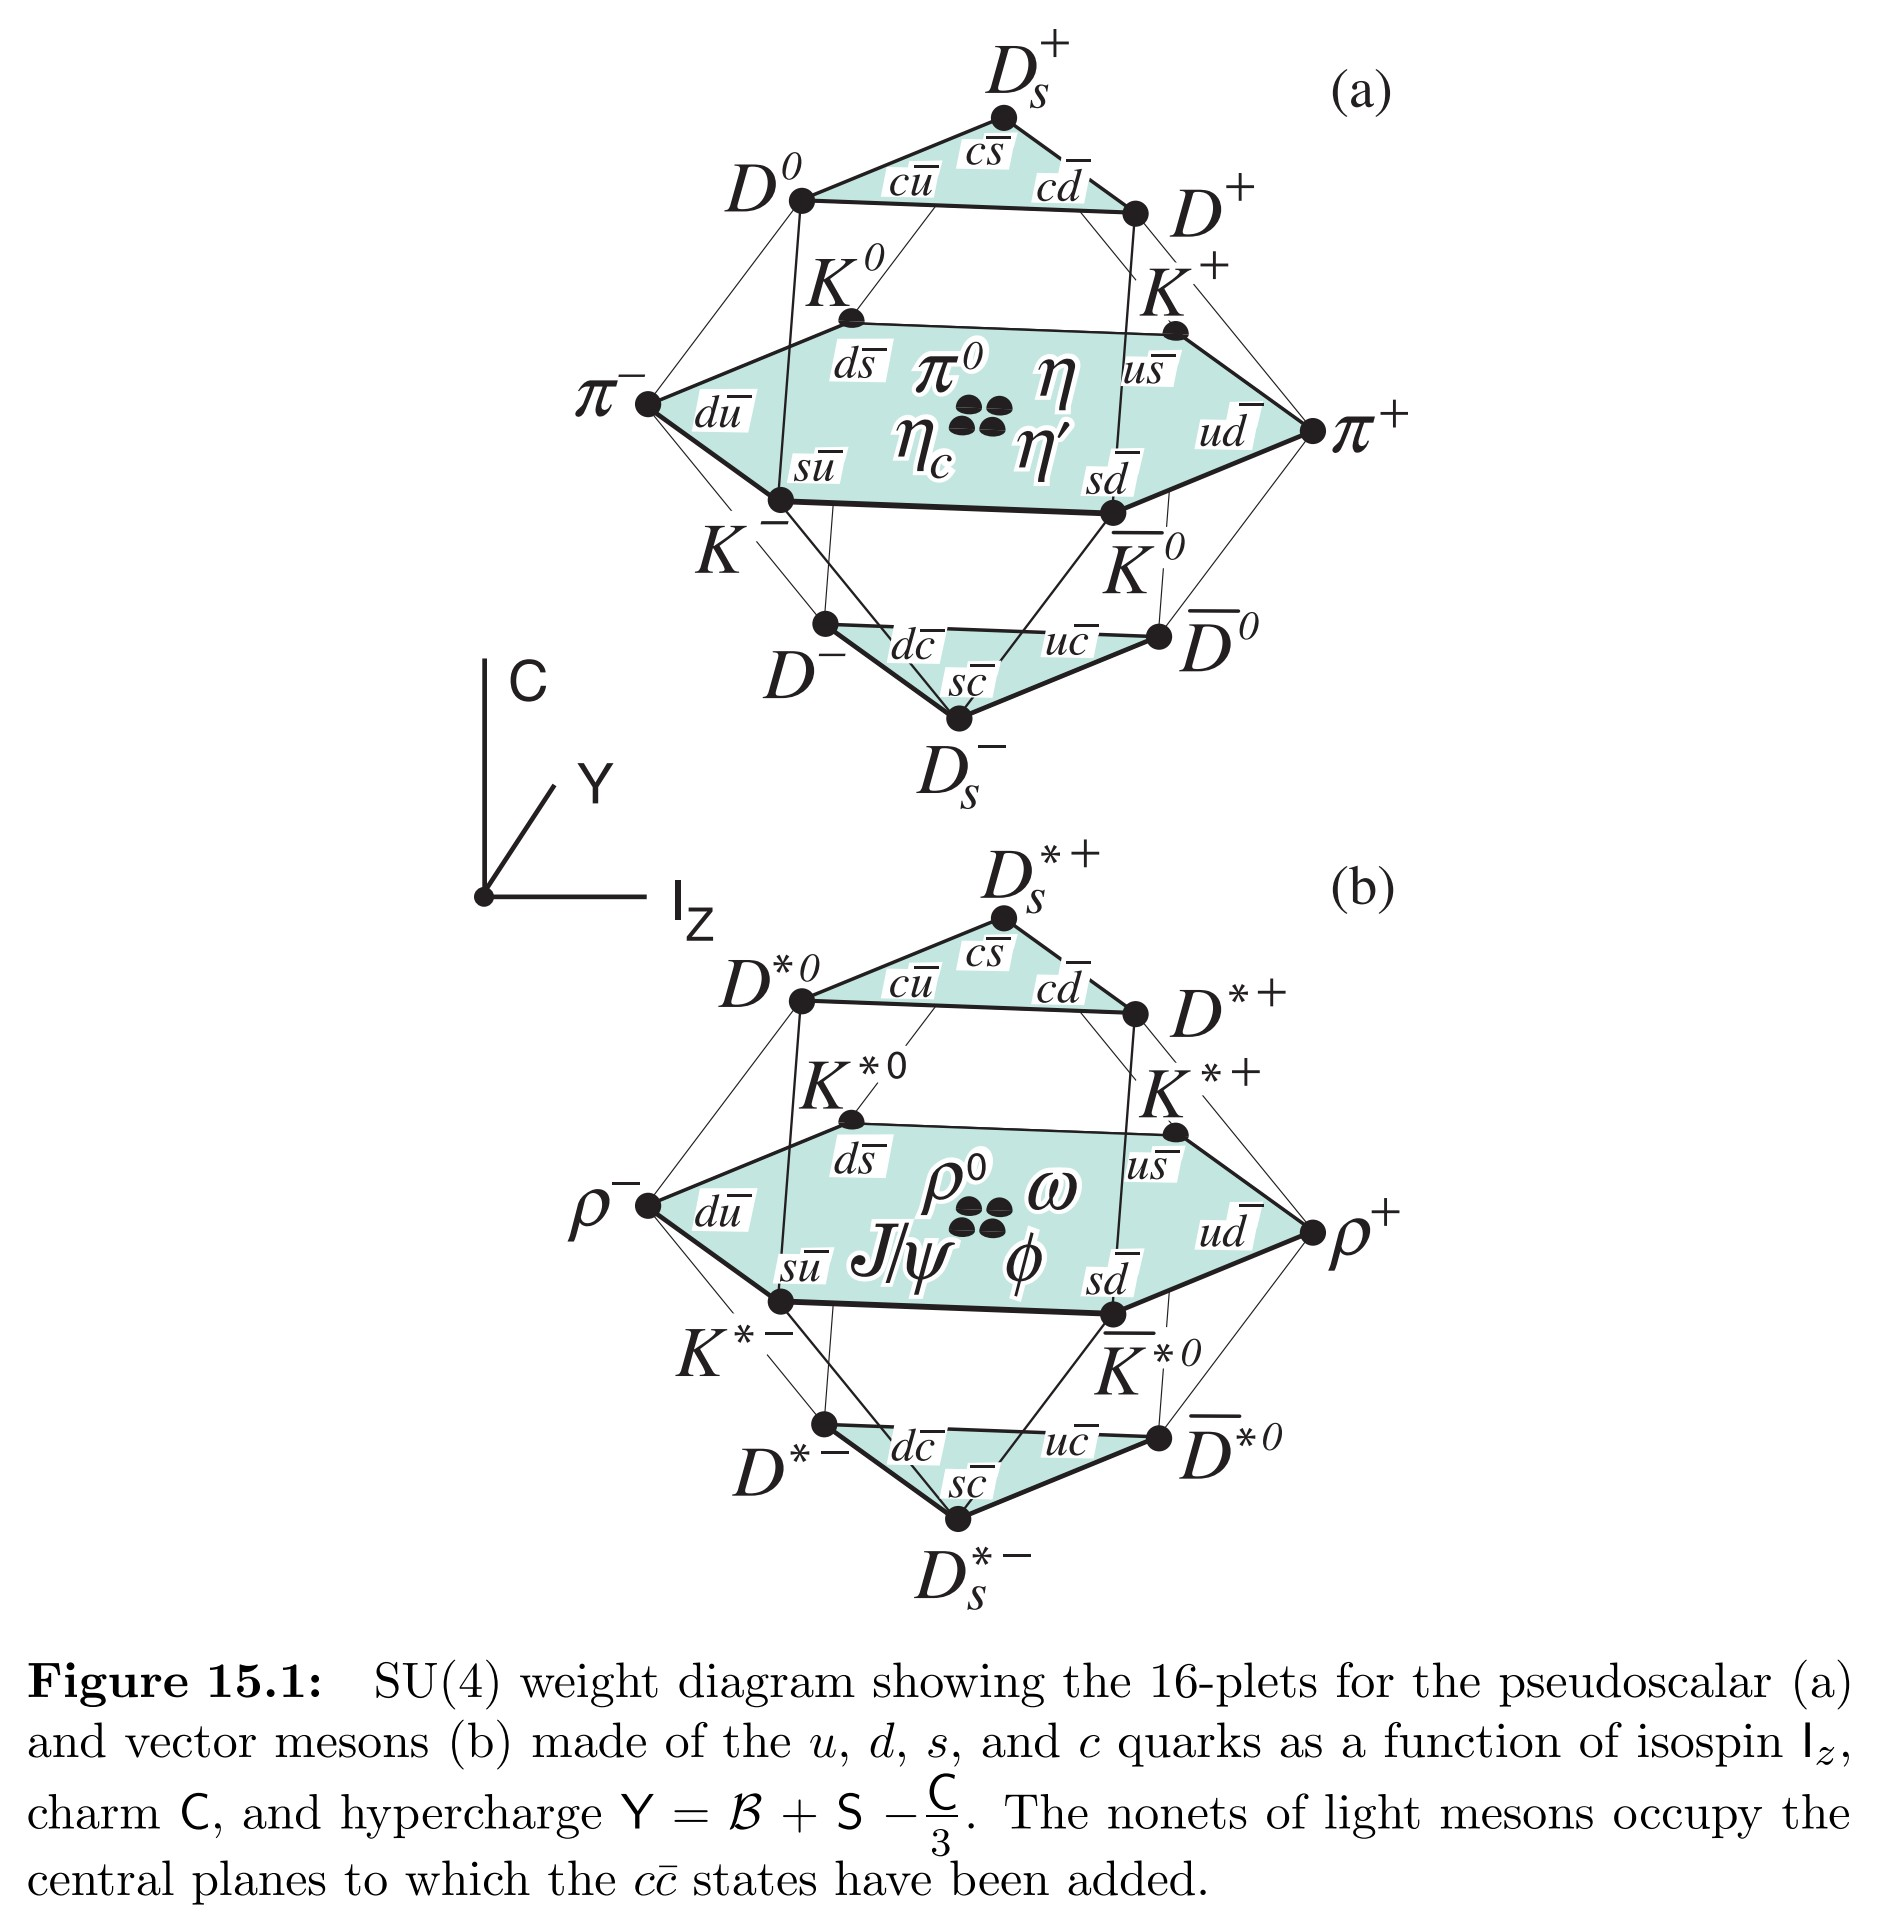
\includegraphics[height=0.9\textheight, width=\linewidth, keepaspectratio]{Images/90f0590a-0e4a-4d62-bd40-0bcce4be9feb.jpg}%\caption{C Amsler, T DeGrand et al 2017 - Quark Model.jpg}
      \figcite{C.Amsler.2017}
    
    \end{frame}


    
    % Bibliography    
    \begin{frame}[allowframebreaks, noframenumbering, plain]{Literaturverzeichnis}
   \printbibliography%[nottype=unpublished]
    \end{frame}

\end{document}
